\documentclass[10pt,landscape,a4paper]{article}
\usepackage{multicol}
\usepackage[landscape]{geometry}
\usepackage{hyperref}
\usepackage[utf8]{inputenc}
\usepackage{minted}
\usepackage{graphicx}
\usepackage[binary-units]{siunitx}
\usepackage[usenames]{xcolor}
\usepackage{ulem}

\geometry{top=0.5 cm,left=1.5cm,right=1cm,bottom=0.5cm}

% Turn off header and footer
\pagestyle{empty}
 
% Redefine section commands to use less space
\makeatletter
\renewcommand{\section}{\@startsection{section}{1}{0mm}%
                                {-1ex plus -.5ex minus -.2ex}%
                                {0.5ex plus .2ex}%x
                                {\normalfont\large\bfseries}}
\renewcommand{\subsection}{\@startsection{subsection}{2}{0mm}%
                                {-1explus -.5ex minus -.2ex}%
                                {0.5ex plus .2ex}%
                                {\normalfont\small\bfseries}}
\renewcommand{\subsubsection}{\@startsection{subsubsection}{3}{0mm}%
                                {-1ex plus -.5ex minus -.2ex}%
                                {1ex plus .2ex}%
                                {\normalfont\footnotesize\bfseries}}
\renewcommand{\paragraph}{\@startsection{paragraph}{3}{\z@}%
                                {-1ex plus -.5ex minus -.2ex}%
                                {-.5em}%
                                {\normalfont\scriptsize\bfseries}}
\makeatother

% Don't print section numbers
\setcounter{secnumdepth}{0}

\setlength{\parindent}{0pt}
\setlength{\parskip}{0pt plus 0.5ex}

% Compact lists
\usepackage{enumitem}
\setlist{nosep}

%Define Colors
\definecolor{reg1}{HTML}{D6B656}
\definecolor{reg2}{HTML}{6C8EBF}
\definecolor{reg3}{HTML}{82B366}

\definecolor{green}{HTML}{82B366}
\definecolor{blue}{HTML}{4a86e8}

%C-Code inline
\newcommand{\prgc}[1]{\mintinline{C}{#1}}

% -----------------------------------------------------------------------

\begin{document}

\footnotesize
\begin{multicols*}{3}

% multicol parameters
% These lengths are set only within the two main columns
%\setlength{\columnseprule}{0.25pt}
\setlength{\premulticols}{1pt}
\setlength{\postmulticols}{1pt}
\setlength{\multicolsep}{1pt}
\setlength{\columnsep}{2pt}

%\section{Zahlensysteme}
\subsection{Stellenwertsystem}

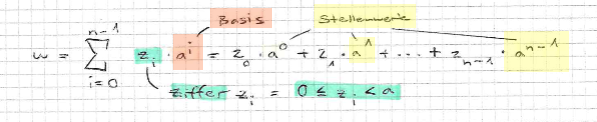
\includegraphics[width = \columnwidth]{stellenwertsystem.PNG}

Nibble = 4 Bit, Oktett = 8 Bit, Byte = Oktett (für uns)

\subsection{Minima/Maxima}
\textbf{unsigned/ohne Vorzeichen}: $0...2^{n}-1$\\
\textbf{signed/mit Vorzeichen}:\\
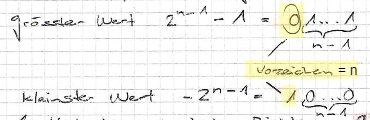
\includegraphics[scale = .75]{zweierkomplement1.PNG}

\subsection{Zweierkomplement}
Allgemein bei -1 alle Bits gesetzt: 1..1\\
Maximum $2^{n-1}-1$ invertiert = 10..01\\
$N(0) = 0$, $2^{n-1} = N(2^{n-1}) = 100..$\\ \\
\textcolor{yellow}{bestimmt Vorzeichen, 0 = +, 1 = -, index = n}

\subsubsection{1. Variante: Subtraktionsverfahren}
$N(b)=2^{n} - b$, b = binäre Zahl\\
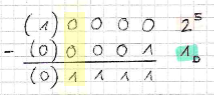
\includegraphics[scale = .5]{zweierkomplement2.PNG}

\subsubsection{2. Variante: Inversionsverfahren}
- 1, invertieren\\
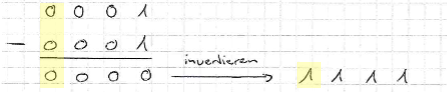
\includegraphics[scale = .5]{zweierkomplement3.PNG}\\
3. Variante: invertieren + 1

%\subsection{Zweierpotenzen}
%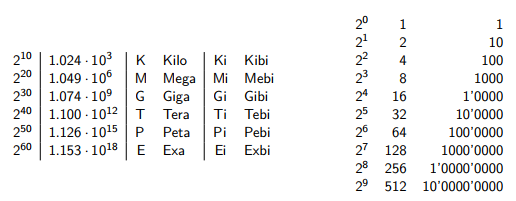
\includegraphics[width = \columnwidth]{zweierpotenzen.PNG}
\hline
\subsection{Logik}
\textcolor{blue}{Funktion}, \textcolor{red}{Parameter/Platzhalter}, \textcolor{green}{Argument}\\
$\textcolor{blue}{f(}\textcolor{red}{x, y}\textcolor{blue}{)} := x \wedge \textcolor{blue}{g (}\textcolor{green}{x,y}\textcolor{blue}{)}$\\ 

\textbf{Anzahl Argumentkombinationen} $2^{n}$, n = Anzahl Argumente

\begin{description}
%\item[unär Funktion]{$f(x) = x$}
%\item[binär Funktion]{$f(x,y) = x \wedge y$}
\item[n-äre Funktion]{$f(x_{0}, .., x_{n-1}) = x_{0} \wedge x_{1} \wedge .. \wedge x_{n-1}$}
\item[nulläre Funktion]{f() = 1}
\end{description}

\subsection{Unäre Funktionen}
\textbf{Identität I(p):} I(x) = x, I(1) = 1, I(0) = 0 oder einfach x\\
\textbf{Negation N(p):} N(1) = 0, N(0) = 1 oder einfach $\neg x$\\
F(p) immer 0 (eigentlich nullär)\\
T(p) immer 1 (eigentlich (nullär)

\subsection{Disjunktion, Konjunktion}
\textbf{Disjunktion:} $\vee$, \textbf{Konjunktion:} $\wedge$\\
Kanonische disjunktive Normalform (KDNF): Alle wahren Zeilen aus Wahrheitstabelle mit $\wedge$ verknüpft

\subsubsection{Dualität}
Dualität: 0 und 1, v und $\wedge$ sind dual zueinander
Ersetzt man in einer korrekten Formel alle 0, 1, ∨ und ∧ durch ihr jeweils duales Element, ist auch diese duale Formel korrekt.

\subsubsection{Regeln}
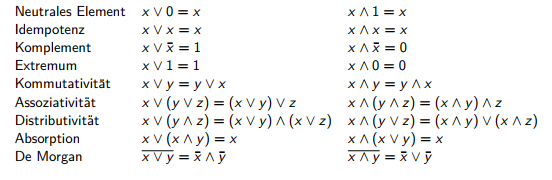
\includegraphics[width = \columnwidth]{regelnkonjdis.PNG}

\subsection{Binäre Funktionen}
\subsubsection{Exklusives Oder}
$x \oplus y$\\
Entweder x = 1 oder y = 1, nicht beides gleichzeitig\\
Negation der Äquivalenz $\neg(x \leftrightarrow y)$\\
Entspricht der Addition zweier Bits ohne Übertrag (Übertrag ist x ∧ y)

\subsubsection{NAND, NOT AND}
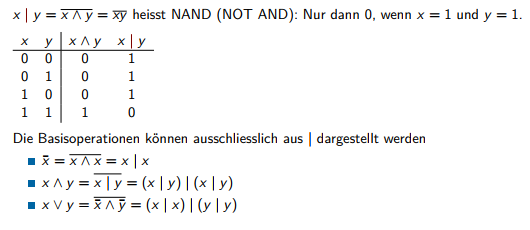
\includegraphics[scale = 0.6]{notand.PNG}

%\section{Prozessor}
%\subsection{Modellierung}
%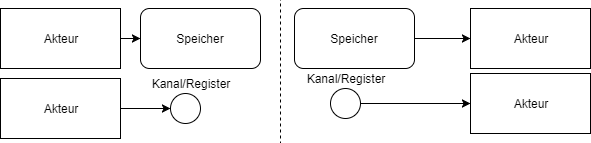
\includegraphics[width = \columnwidth]{modellierung.png}
%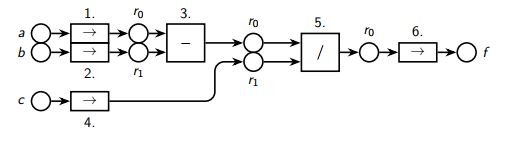
\includegraphics[width = \columnwidth]{bsp_modellierung.PNG}
%\textbf{1.} $a \rightarrow r0$ 
%\textbf{2.} $b \rightarrow r1$ 
%\textbf{3.} $r0 - r1 \rightarrow r0$ 
%\textbf{4.} $c \rightarrow r1$ 
%\textbf{5.} $r0 : r1 \rightarrow r0$ 
%\textbf{6.} $r0 \rightarrow f$


%Menge aller Maschinencodes = Befehlssatz, instruction set, Prozessoren mit gleichem Befehlssatz = Prozessorfamilie/Architektur

\subsection{Prozessor-Zyklus}
1. Prozessor fordert Wert von der Adresse an, die im Befehlszeiger steht.
2. Prozessor decodiert Instruktion aus Wert.
3. Prozessor wählt den zur Instruktion gehörenden Baustein aus.
4. Aktiver Baustein decodiert Parameter aus Wert.
5. Aktiver Baustein liest aus den Registern.
6. Aktiver Baustein führt Berechnung aus.
7. Aktiver Baustein schreibt in die Register.
8. Prozessor erhöht Befehlszeiger entsprechend der Länge der Instruktion.

%\subsection{Definition Prozessor}
%automatische Maschine mit internem Zustand(Register), Schnittstelle für Adressen und Daten,
%fordert automatisch Daten/Instruktionen an, interne/externe Zustand kann geändert werden
\hline

\subsection{Assembler}
assembly = language, assembler, Compiler

\subsection{Byte-Order}
\textbf{16 Bit:}\\
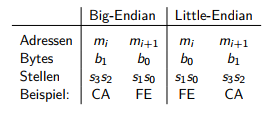
\includegraphics[scale = 1]{endian.PNG}\\
\textbf{32 Bit:}\\
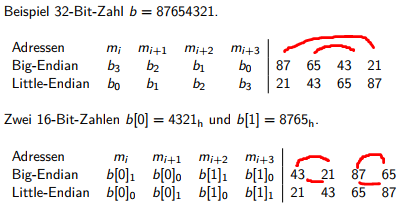
\includegraphics[scale = 1]{byteorder32.PNG}

Byte 1 Byte / 8 Bit, db 0x35
Word 2 Byte / 16 Bit, dw 0x2135 $\leftrightarrow$ db 0x35, 0x21\\
Doubleword 4 Byte / 32 Bit, dd 0x2135 $\leftrightarrow$ db 0x35, 0x21, 0x00, 0x00\\
Quadword 8 Byte / 64 Bit, dq\\
Double Quadword 16 Byte / 128 Bit

\subsection{Register}

instruction pointer: ip in 16-bit, eip in 32-bit, rip in 64-bit

\includegraphics[scale = 0.3]{assembler.png}\\
\begin{tabular}{lllll}
1 & RAX     & \textcolor{reg1}{EAX}     & \textcolor{reg2}{\textit{AX}} & \textcolor{reg3}{AL}\\
2 & RBX     & \textcolor{reg1}{EBX}     & \textcolor{reg2}{\textit{BX}} & \textcolor{reg3}{BL}\\
3 & RCX     & \textcolor{reg1}{ECX}     & \textcolor{reg2}{\textit{CX}} & \textcolor{reg3}{CL}\\
4 & RDX     & \textcolor{reg1}{EDX}     & \textcolor{reg2}{\textit{DX}} & \textcolor{reg3}{DL}\\
5 & RSI     & \textcolor{reg1}{ESI}     & \textcolor{reg2}{SI} & \textcolor{reg3}{SIL}\\
6 & RDI     &  \textcolor{reg1}{EDI}    & \textcolor{reg2}{DI} & \textcolor{reg3}{DIL}\\
7 & RSP     & \textcolor{reg1}{ESP}     & \textcolor{reg2}{SP} & \textcolor{reg3}{SPL}\\
8 & RBP     & \textcolor{reg1}{EBP}     & \textcolor{reg2}{BP} &  \textcolor{reg3}{BPL}\\
9 & R8-R15  & \textcolor{reg1}{R8D-R15D} & \textcolor{reg2}{R8W-R15W} & \textcolor{reg3}{R8L-R15L}
\end{tabular}\\
1. Accumulator, 2. Datenpointer, 3. Counter für Schleifen, Stringoperationen, 4. Pointer für I/O-Operationen,
5. Quelindizes für Stringoperationen, 6. Zielindizes für Stringoperationen, Exitcode, 7. Stackpointer, Adresse des allozierten Stacks,
8. Basepointer, Adresse innerhalb des Stacks, Basis des Rahmens der Funktion , 9. Zusätzliche Register

\textcolor{reg2}{\textit{Obererer 8-Bit Teil kann separat verwendet werden: AH, BH, CH, DH}}\\
Operationen auf \textcolor{reg3}{8 Bit} und \textcolor{reg2}{16-Bit-Registerteil} ändern den Rest des Registers nicht,
Bei Operationen auf \textcolor{reg1}{32-Bit Ebene} wird der obere Teil auf 0 gesetzt

\subsection{Adressierungsmodi}
Die Adresse der Speicherstelle folgt unmittelbar(Displacement): mov rax, [0x1000]\\
Die Adresse der Speicherstelle steht in einem Register (Base): mov rax, [rcx]\\
(Index * Scale): Index ist ein Register und Scale ist 1, 2, 4, oder 8, mov rax, [rbx * 4]\\

Referenz = Wert der gespeicherten Adresse wird eingesetzt\\
2E0_{h} = 2\\
rax = 2E0_{h}\\
mov rbx, [rax] $\leftrightarrow$ mov rbx, 2

\subsubsection{Label}
somedata: db 'Hallo'\\
start: mov rax, rbx

Label wird nicht übersetzt, wird mit dem Offset A(\textit{label}) des nachfolgenden Befehls assoziiert\\
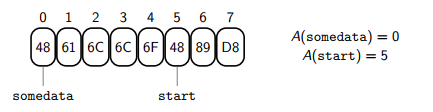
\includegraphics[scale = 1]{label.PNG}

\subsubsection{Arrays}
\textcolor{red}{Startadresse},
Offset O_{\textcolor{red}{a}}(\textcolor{green}{index}) = \textcolor{green}{Index} $ \cdot $ \textcolor{blue}{Variablengrösse in Byte (Byteadressierung)}

move rax, 0\\ 
add rax, [\textcolor{red}{a} + \textcolor{green}{0} *  \textcolor{blue}{8}]\\
add rax, [\textcolor{red}{a} + \textcolor{green}{1} * \textcolor{blue}{8}]\\
add rax, [\textcolor{red}{a} + \textcolor{green}{2} * \textcolor{blue}{8}]\\
move [r], rax 

\subsection{Arithmetische und logische Operatoren}
Befehle können unterschiedlich lang sein $\rightarrow$ Sequenz muss Befehl für Befehl durchgegangen werden\\
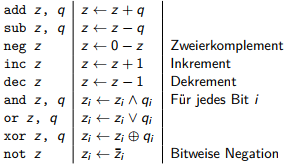
\includegraphics[scale = 1]{operatoren.PNG}

\subsection{Shifting}
\subsubsection{Links-Shift}
Multiplikation einer Binärzahl mit $2^{m}$\\
um m-Stellen nach links verschieben + mit m-Nullen auffüllen\\
1111 Linksshift um $2^{1}$ = 1111\textcolor{red}{0}  

\subsubsection{Rechts-Shift}
Division einer Binärzahl um $2^{m}$\\
um m-Bits nach rechts verschoben + links mit 0 auffüllen\\
1111 um $2^{1}$ \textcolor{red} = {0}111

\subsubsection{Sign-Extension}
Statt \textcolor{red}{0} wird überall \textcolor{red}{1} reinkopiert\\
Rechtsshift mit Signextension = Arithmetischer Rechts-Shift

\subsubsection{Rotate}
Rotates füllen mit den \textcolor{red}{ursprünglichen Bits} auf

\subsubsection{Befehle}
i = Konstante oder Register \textcolor{reg3}{CL}\\
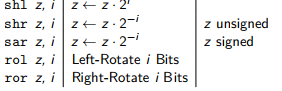
\includegraphics[scale = 0.5]{shifts.PNG}

\subsection{Multiplikation}
\subsubsection{unsigned}
Ergebnis einer Multiplikation benötigt doppelt so viele Bits wie einzelne Operanden\\
Also 2n Bit

\subsubsection{signed}
Vorzeichen explizit berücksichtigen!

\subsubsection{Befehle}
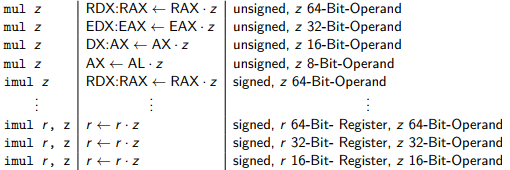
\includegraphics[scale = 0.5]{multiplikation.PNG}

\subsection{Division}
sehr langsam $\rightarrow$ für Zweierpotenzen durch Rechts-Shift ersetzen\\
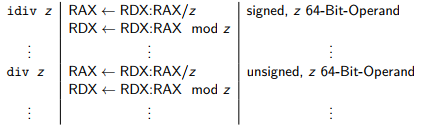
\includegraphics[scale = 0.5]{division.PNG}

\begin{multicols}{2}
\subsection{Relative Sprünge}
JMP zahl = RIP$\leftarrow$RIP + zahl\\
JMP label = RIP$\leftarrow$label\\
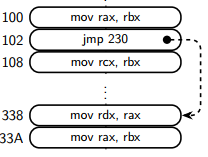
\includegraphics[scale = .5]{relativ.PNG}
\vfill\null
\columnbreak
\subsection{Flags}
gemeinsames Register RFLAGS
\begin{description}
\item[Carry Flag - CF]{Überlauf unsigned}
\item[Overflow Flag - OF]{Überlauf signed}
\end{description}
werden immer beide bestimmt
\begin{description}
\item[Zero Flag - ZF]{Resultat = 0}
\item[Sign Flag - SF]{MSB des Resultats}
\item[Parity Flag - PF]{niederwertigste Byte = gerade Anzahl 1}
\end{description}
\end{multicols}

\subsubsection{Condition Codes}
\begin{tabular}{lll}
\textcolor{blue}{CC} & Name &  Flags\\
\hline
\textcolor{blue}{A}   & Above             & CF = 0 und ZF = 0\\
\textcolor{blue}{AE}  & Above or Equal    &  CF = 0\\
\textcolor{blue}{B}   & Below             & CF = 1\\
\textcolor{blue}{BE}  & Below or Equal    & CF = 1 oder ZF = 1\\
\textcolor{blue}{E}   & Equal             & ZF = 1\\
\textcolor{blue}{G}   & Greater           & ZF = 0 and SF = OF\\
\textcolor{blue}{GE}  & Greater or Equal  & SF = OF\\
\textcolor{blue}{L}   & Less              & SF $\neq$ OF\\
\textcolor{blue}{LE}  & Less or Equal     & ZF = 1 und SF $\neq$ OF\\
\textcolor{blue}{PE}  & Parity Even       & PF = 1\\
\textcolor{blue}{PO}  & Parity Odd        & PF = 0
\end{tabular}


\textbf{einbuchstabigen \textcolor{blue}{CC}: }\textcolor{blue}{C} $\leftrightarrow$ CF = 1\\
\textbf{negierter \textcolor{blue}{CC}: }N\textcolor{blue}{C} $\leftrightarrow$ CF = 0

\subsubsection{cmp}
cmp rax, rbx berechnet RAX – RBX, verwirft Ergebnis, setzt Flags

\subsubsection{Bedingte Anweisungen}
CMOV\textcolor{blue}{cc}: Conditional MOV, J\textcolor{blue}{cc}: Conditional JMP, SET\textcolor{blue}{cc}: Schreibt 1 ins 8-Bit grosse Ziel, wenn \textcolor{blue}{CC} erfüllt, sonst 0 

\subsection{Programmstart/-ende}
\textbf{Entrypoint} = \_start:

Intel Prozessoren haben Privilege-Levels: 0 = OS, 3 = Programme, deshalb:\\ 
mov rax, 60; Funktionscode\\
mov rdi, 0; weitere Argumente, hier Exitcode 0\\
syscall; Handler für Syscalls -$>$ Unter-Handler für 60

\subsection{Stack, Funktionen, Variablen}
\textbf{call} x legt die Rucksprungadresse auf den Stack und springt dann zu x\\
\textbf{ret} nimmt die Rucksprungadresse vom Stack und springt dahin\\
\textbf{Parameter und lokale Variablen} werden je nach Calling Convention auf dem Stack
oder in Registern abgelegt\\
\textbf{Parameter} sind lokale Variablen, die vom Caller initialisert werden\\
\textbf{Globale Variablen} verhindern rekursive (allg. re-entrante) Funktionen, sind fix im Speicher mit eigener Adresse

\hline
\subsection{C Toolchain}
1. Präprozessor\\
2. Compiler\\
3. Assembler Assemblerdatei .asm$\rightarrow$Objektdatei/Binärsequenz .o\\
4. Linker mehrere Objektdateien/Binärsequenzen $\rightarrow$Executable
\subsubsection{Objekt-Datei}
Enthält Binärsequenzen\\
Symboltabelle Bestandteil von Obj-Datei::\\
\begin{tabular}{llll}
 \textcolor{green}{0000   &   &*UND*  &y}\\
 \textcolor{green}{0000   &   &*UND*  &g}\\
 \textcolor{blue}{\textit{0008}   &g  &.text  &x}\\
 \textcolor{blue}{\textit{0010}   &g  &.text  &f}
\end{tabular}

\textit{Offset}
\textcolor{blue}{Exportierte Symbole: global deklarierte Label x, f}
\textcolor{green}{Importierte Symbole: extern deklarierte Label = *UND*}

In Objektdatei, Stellen mit Symbolen 0x0, da Adresse noch nicht bekannt

\subsubsection{Executable}
Jedes Symbol erhält einen eigenen, festen Platz im Executable

\subsubsection{Präprozessor}
\textbf{1. Durchlauf}\\ 
Entfernen aller Kommentare, fortgesetzte Zeile $\rightarrow$ in eine Zeile\\
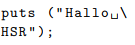
\includegraphics[scale = .5]{praeprozessor1.PNG}
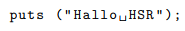
\includegraphics[scale = .5]{praeprozessor2.PNG}

\textbf{2. Durchlauf, Tokenization}\\ 
\textbf{Bezeichner}\\
\sout{Sonderzeichen}, Beginn mit \_/A-Za-z\\
\textbf{Präprozessor-Zahlen: }\\
beginnt mit Ziffer, Bsp: 0, 1, 0123, 0x1234, .\prgc{05}, \prgc{0_.0}\prgc{*(nicht gueltig in C)*}, 
\prgc{0xE+12}*(wird nicht als 0xE + 12 interpretiert!)*, \prgc{p+}, \prgc{P+}, \prgc{p-}, \prgc{P-}, ungültige Zahlen $\rightarrow$ vom Compiler entdeckt\\
\textbf{String- und Character-Literale}\\
immer zusammengefasst, " escapen: \textbackslash",' escapen: \textbackslash'\\
\textbf{Operatoren und Satzzeichen (punctuators)}\\
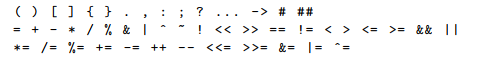
\includegraphics[width = \columnwidth]{op.PNG}\\
Der Präprozessor ist greedy:\\
ist \prgc{a+++++b} nicht \prgc{a++ + ++b} sondern \prgc{a++ ++ +b} (ungültiger Ausdruck)\\

Whitespace (Leerschlag, Zeilenumbruch, Tabulator) trennt Token voneinander, aber
nicht alle Token mussen durch Whitespace getrennt werden, z.B. a+b$\leftrightarrow$\fbox{a} \fbox{+} \fbox{b}.

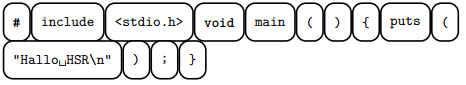
\includegraphics[width = \columnwidth]{token.PNG}

\textbf{3. Durchlauf}\\
Präprozessor-Direktiven ausführen, Makros durch Expansion ersetzen\\
\# nächste Token als direktive\\
Direktiven: \prgc{include header}, \prgc{define makro}, \prgc{if}, \prgc{else}, \prgc{endif}\\

\\\#\prgc{include}:\\
\#\prgc{include <file.h>} sucht nur in den Systemverzeichnissen\\
\#\prgc{include "file.h"} erst im aktuellen Verzeichnis und dann in den
Systemverzeichnissen\\
1. Präprozessor fuhrt Durchläufe 1 bis 3 für file.h durch\\
2. Präprozessor setzt Arbeit nach der Direktive in Orignaldatei fort

\textbf{Objektartige Makros:} \#\prgc{define XYZ 123}\\

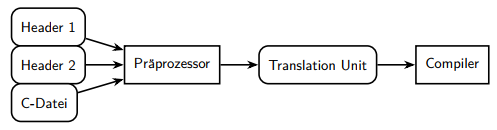
\includegraphics[width = \columnwidth]{include_mechanismus.PNG}

\subsubsection{Variablen}
globale Variable analog Assembler, Speicher wird fix reserviert, Grösse durch Typ bestimmt\\
Bezeichner = Label auf Assembler-Ebene

Intialisierung:\\
\prgc{int x = 15;} $\leftrightarrow$ x : dd 15\\
Ohne Initialwert$\rightarrow$mit 0 initialisiert\\
Globale Variablen werden standardmässig exportiert (wie Assembler)\\

Globale Variablen aus anderen Dateien: \prgc{extern int c;}

\subsubsection{Objekt} 
zusammenhängender Speicherbereich, Inhalt kann als Wert interpretiert werden
\textbf{Objektgrösse bestimmen: } \prgc{sizeof(T)}

\subsubsection{Basistypen}
\begin{tabular}{ll}
\prgc{char}                     & mind. 8 Bit (nach Impl. signed/unsigned)\\
\prgc{[signed] short [int]}     & mind. 16 Bit\\
\prgc{[signed] int}             & mind. 16 Bit\\
\prgc{[signed] long [int]}      & mind. 32 Bit\\
\prgc{[signed] long long [int]} & mind. 64 Bit
\end{tabular}
Somit default-mässig signed\\
unsigned muss sonst strikt angegeben werden

\subsubsection{Pointer-Typen}
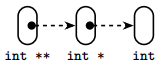
\includegraphics[scale = .5]{pointertypen.PNG}

\subsubsection{Referenzoperator}
\prgc{&a} = Adresse der Variable \prgc{a}\\
\prgc{T*} ist der Typ des Ausdrucks \prgc{&a}

\subsubsection{Dereferenzoperator}
\prgc{*} wandelt Adress-Ausdruck in Ausdruck bezogen auf Inhalt um\\ \\
*\&a ergibt wieder a und \&*b ergibt wieder b (wenn b eine Pointervariable ist)\\

Testen auf Null-Pointer: \prgc{if (px == 0)}\\

Funktionspointer:
\begin{minted}{C}
int f (int x, int y);
int (*p) (int, int) = &f;
p = g; //andere Funktion zuweisen
int i = (*p) (1,2);
int j = p (3,4); //Alternativer Aufruf
\end{minted}

\subsubsection{Arrays}
Bezeichner eines Arrays $\rightarrow$ Pointervariable\\
Jeder Pointer kann im Array verwendet werden:
Mit Elementtyp T ist \prgc{a[index]} äquivalent zu \prgc{a + sizeof(T) * index}

\subsubsection{Structs}
\begin{minted}{C}
struct T //Tag für Wiederverwendung
{int x; int y;}; 
\end{minted}
\begin{minted}{C}
struct T t, u;
\end{minted}
belegt gleichen Speicherplatz wie \prgc{int x; int y;}einzeln\\
Zugriff: \prgc{t.x = t.y}\\
\prgc{x} gleiche Adresse wie Struct\\
Member müssen im Speicher nicht dicht liegen (Padding möglich)\\
\textbf{Pointer auf Structs: }\prgc{struct T* z; t->x = t->y;}\\

\textbf{Zuweisungen eines Structs auf einen anderen $\rightarrow$ ganzer Inhalt kopiert(nicht nur Referenz)}

\subsubsection{Union}
zur Verhinderung von Casts, 
ähnlich wie Structs, 
Start der Adressen der Elemente = Start der Adresse der Union 
Grösse der Union = Grösse des grössten Elements
\prgc{union U{//Elemente}}

\subsubsection{Funktionen}

\begin{minted}{C}
void f();
f(1,2,3); // OK
\end{minted}

Parameter abhängig von Calling Convention in Registern/Stack übergeben\\
Immer \textbf{Call by value}\\

\textbf{Pointer: } \prgc{int f (int* f)}, 
Call by Reference emuliert\\

\textbf{Arrays: }
Arrays werden als Pointer intepretiert/übergeben
\prgc{f(int x[], int len)} = \prgc{f(int* x, int len)}

\textbf{Structs: }
ganzer Struct als Argument kopiert, mit Struct Pointer $\rightarrow$analog Java

\subsubsubsection{Type-Definitionen}
anderer Bezeichner für denselben Typen definieren\\
\prgc{typedef struct {my_int x; } T;}\\  %String Beispiel einfügen!!

\subsubsection{\prgc{printf}}
indirekte Ausgabe über stdout, Ausgabe erst wenn Buffer voll\\
\prgc{write} ist direkte Ausgabe\\
sofortige Ausgabe: \prgc{fflush(stdout)}

vom Stack eingelesen:\\
\begin{tabular}{ll}
\%i      & \prgc{sizeof(int)}Bytes\\
\%X      & \prgc{sizeof(int)}Bytes als Hex\\
\%li     & \prgc{sizeof(long)}Bytes\\
\%lli    & \prgc{sizeof(long long)}Bytes
\end{tabular}

als Pointer:\\
\begin{tabular}{ll}
\%p      & \prgc{sizeof(void *)}Bytes \\
\%s      & \prgc{sizeof(char *)}Bytes auf null-terminierten String 
\end{tabular}


\hline
\subsection{Cache}
\subsection{Mittlere Zugriffszeit}
\textbf{Cache-Hit} Gesuchte Adresse ist im Cache\\
\textbf{Cache-Miss} Gesuchte Adresse ist nicht im Cache\\
$T_{C}$ Zugriffszeit auf den Cache\\
$T_{M}$ Zugriffszeit auf den Hauptspeicher\\
$p_{C}$ Wahrscheinlichkeit eines Cache-Hits (wegen Lokalitätseffekt oft $>$ 0.9)\\

Erwartungswert E(T) der Cache-Zugriffszeit T:\\
$E(T) = p_{C} \cdot T_{C} + (1 - p_{C}) \cdot T_{M}$

\subsection{Fully Associative Cache (FAC)}
Eintrag i besteht jeweils aus \textcolor{red}{Adresse $a_i$} und und \textcolor{blue}{Datenbyte $d_i$ = [$a_i$]}

\subsubsection{Cachezeilen à 64 Byte}
nur die Adresse des ersten Bytes wird gespeichert\\
\textbf{Total Einträge: }Grösse des Caches(\textcolor{reg1}{b}) / \textcolor{reg2}{64 Einträge}\\
\textcolor{reg2}{64 = $2^\textcolor{reg3}{{6}}$}\\
\textbf{n-Bit Adresse: }\textcolor{red}{ $t_i$: oberen n-\textcolor{reg3}{6} Bit} + Offset(untere \textcolor{reg3}{6} Bit)\\
\textbf{Overhead: }$2^{n - \textcolor{reg3}{6}} \cdot \textcolor{reg1}{b}$

\subsubsection{Lookup}
Zu jeder Zeile ein \textcolor{yellow}{Hardware-Baustein $c_i$}, der überprüft \textcolor{green}{t} = \textcolor{red}{$t_i$}\\
Überprüfung wird parallel gemacht\\
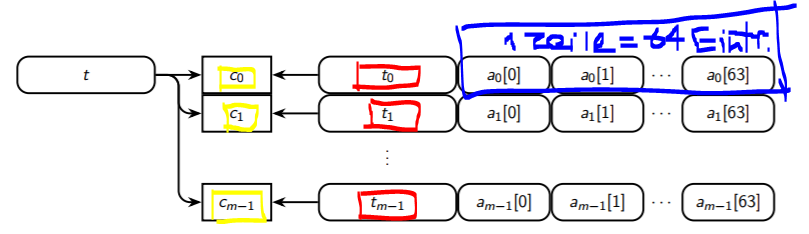
\includegraphics[scale = 0.5]{fac.PNG}

+ Lokalitätsprinzip bestmöglich ausgenutzt\\
- Lookups benötigen viel Hardware (\textcolor{yellow}{$c_i$}) und sind teuer

\subsection{Direct-Mapped Cache (DMC)}
Anzahl Einträge/Zeilen = $2^\textcolor{blue}{s}$\\
eine Cachezeile nur an einem einzigen Ort möglich\\
\textcolor{brown}{Eintrag wird durch die untersten \textcolor{blue}{s} Bit des Tags \textcolor{red}{t} bestimmt}\\
\textcolor{red}{$t_i$} = \textcolor{green}{$t'_i$}$\cdot 2^{\textcolor{blue}{s}} + \textcolor{brown}{i}$\\
\textcolor{green}{gespeichert wird nur das reduzierte Tag $t'_i$}, \textcolor{brown}{i} wird abgeleitet
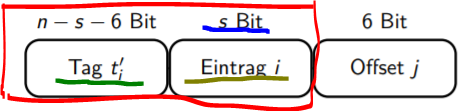
\includegraphics[scale = 0.5]{dmc.PNG}

\subsubsection{Lookup}
ein einziger Vergleichsbaustein\\
Überprüfung t' = \textcolor{green}{$t'_i$}\\
\textbf{Vollständige Adresse: }$(\textcolor{red}{t'_i} \cdot 2^{\textcolor{blue}{s}} + \textcolor{brown}{i}) \cdot 2^{6} + j$

+ einfach zu implementieren
+ sehr schneller Lookup
- viele Kollisionen ($1234_h$, $AB34_h$ bei s=8 gleicher Eintrag)

\subsection{Set-Associative Cache}
parallele Verwendung von \textcolor{blue}{k} Direct-Mapped Caches\\
Jede Cachezeile kann in \textcolor{blue}{k} Einträgen gespeichert werden\\
Anzahl Set = \textcolor{blue}{k}\\
Jeder DMC = WAY\\
Set-Nummer = Nummer des Eintrags \textcolor{brown}{i}\\
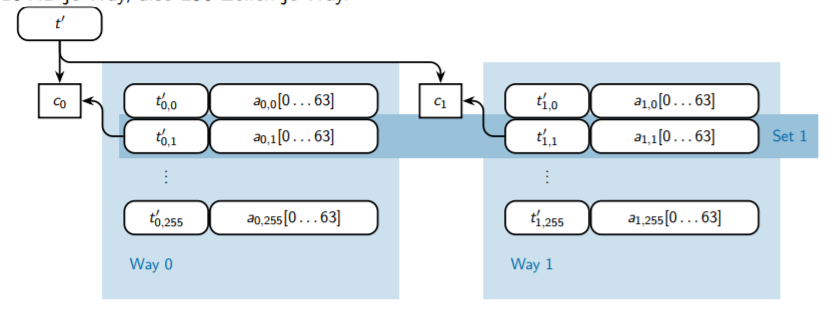
\includegraphics[scale = 0.5]{set-associative.PNG}\\

\textit{ Wie viele Speicherstellen des Hauptspeichers werden jeweils auf dieselben Cacheeinträge
abgebildet?}
$\frac{Grösse RAM \cdot Anz.Ways}{Gesamtgr. Cache}$ = Anteil Hauptspeicher à Anz.Ways Stellen


%guter Kompromiss,
weniger komplex als FAC,
weiniger Kollisionen als DMC,
Genau so schnell wie FAC und DMC

\hline
\subsection{Random Access Memory (RAM)}
\subsection{Heap/Stack}
Heap: Speicherbereich für vollständig dynamischen Speicher\\
Nur \underline{explizite} Speicherfreigabe durch OS vorgesehen:\\
\textbf{Reservieren: }\prgc{void * malloc (unsigned int s)}\\
Reserviert Speicherblock der Grösse s\\
gibt Adresse des allozierten Speicherblocks zurück\\
\textbf{freigeben: }\prgc{void free (void* p)}\\
Grösse wird häufig direkt vor Block angegeben: \prgc{*(p - x)}\\ 

\textbf{Interne Fragmentierung: }Heap reserviert grösserer Speicherblock als angefragt
\textbf{Externe Fragmentierung: }Programm reserviert immmer wieder Speicher, gibt unregelmässig frei

\subsection{Feste Blockgrösse}
\textbf{Dezentrale Speicherung: }Überläufe
\textbf{Zentrale Speicherung: }Speicherplatz muss extra reserviert werden 
\textbf{Bitlisten: }0 Block ist frei, 1 verwendet
\textbf{Verkettete Listen: }Status(frei?), Start(Adresse erster Block), Size(Anzahl Blöcke), Next(Pointer nächstes Listenelement) |
freie Elemente$\rightarrow$zusammengeführt

\subsubsection{Suchalgorithmen}
\textbf{First Fit:} Wählt erste passende Lücke am Anfang
\textbf{Next Fit:} Wählt erste passende Lücke nach zuletzt reserviertem Bereich
\textbf{Best Fit:} Durchsucht alle Lücken und wählt die kleinste passende aus
\textbf{Worst Fit:} Durchsucht alle Lücken und wählt die grösste aus

\subsubsection{Grössenklassen/Quickfit}
Bereiche nur in bestimmten Grössen zur Verfügung (Zahlen, Zweierpotenzen..),
freie Bereiche in Liste, \textbf{Quickfit: }wählt kleinstpassenden aus Liste

\subsubsection{Buddy-System}
Wird ein $2^{\textcolor{red}{k}}$-Bereich in zwei $2^{\textcolor{green}{k-1}}$-Buddys geteilt,  \textcolor{green}{müssen deren Startadressen die untersten k-1 Bits = 0}\\
Die Startadresse des einen Buddys ist a\\
Die Startadresse des anderen Buddys ist a mit einer 1 an Bit \textcolor{red}{k}\\
\textit{Bsp. k=8 $\rightarrow$Buddies 1. Bereich: \textcolor{red}{0}\textcolor{green}{000'0000}...0111'1111, 
\\2. Bereich: \textcolor{red}{1}\textcolor{green}{000'0000}...1111'1111\\}
wenn gleich gross \& einziger Unterschied bei \textcolor{red}{k} $\rightarrow$ Buddies 

\subsubsection{Objekt-Pools}
Speicherbereich fester Grösse(Page) in kleinere Bereiche mit gleicher
Grösse unterteilt(Objekte), keine Rekombi bei Rückgabe, 
Mehr Objekte benötigt?$\rightarrow$neue Page, Freie Objekte in Freiliste\\

%\section{Virtueller Speicher | Hardware}
\hline
\subsubsection{Memory Management Unit (MMU)}
%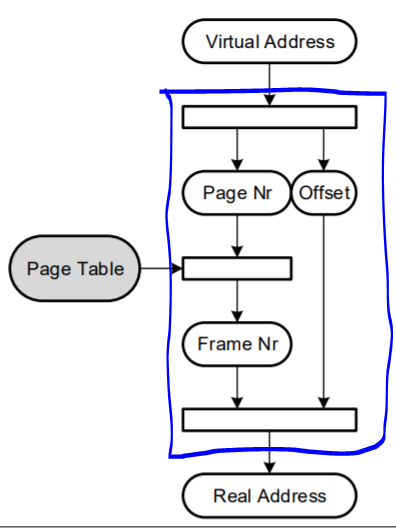
\includegraphics[scale = 0.3]{mmu.PNG}
Pro Prozess eine Page-Table

\subsubsection{Single-Level Page-Table}
ein Eintrag pro Page
+ Lookup sehr schnell $\rightarrow$ Index = PageNumber

\subsubsection{Two-Level Page-Table}
Page Number wird aufgeteilt: Directory Index (nur eine!), Page Table Index (zweidimensionales Array)\\

\textbf{Translation Lookaside Buffer: }Cache für häufig benötigte Mappings
\textbf{Inverted Page-Table: }Pro Frame ein Eintrag, schlimmenstenfalls alle Einträge durchsuchen
\textbf{Hashed Page-Table: }Page Number als Key, gleicher Hash?$\rightarrow$Linked List

\subsubsection{Interprozesskommunikation (IPC)}
\textbf{Shared Memory: }
Prozesse teilen sich Speicher,
+ Kaum Overhead,
- Aufhebung des Schutzes (Bufferoverflow)
\textbf{Message Passing: }
OS kopiert Daten zwischen Prozessen, 
+ Prozesse können sich nicht direkt beeinflussen
- Overhead\\

%\section{Virtueller Speicher | Hardware}
\hline
\subsection{Paging}
MMU setzt A-Bit/«Accessed»|R/Referenced bei jedem Zugriff auf Page,
D-Bit/«Dirty»|M/Modified bei jedem Schreibzugriff auf Page$\rightarrow$zurückschreiben in HDD
%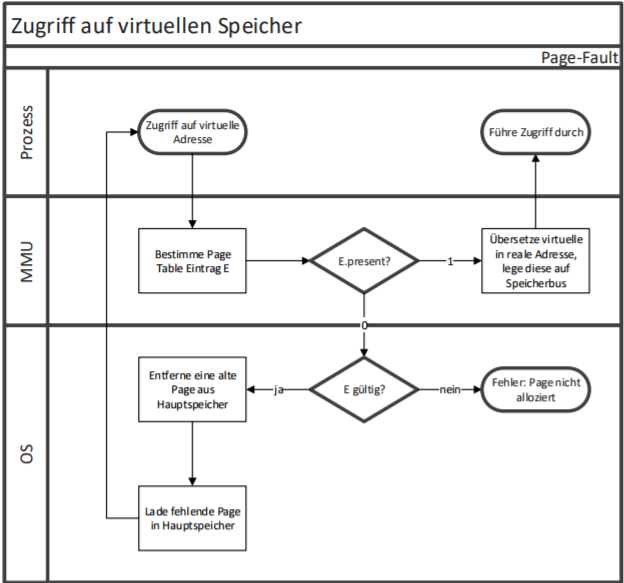
\includegraphics[scale = 0.5]{zugriff.PNG}

\subsection{Dreschen/Häufiges Pagen}
Hauptspeicher viel zu klein/zu viele Prozesse$\rightarrow$mehr Hauptspeicher, 
Beschränkung Anz. Prozesse, 
Verminderung Paging-Strategien

\subsection{Ladestrategien RAM$\leftarrow$HDD}
\textbf{Demand Pagaing: }Laden auf Anfrage, + min. Aufwand, - lange Wartezeiten
\textbf{Prepaging: } Seiten frühzeitig geladen
\textbf{Demand Paging mit Prepaging: }wie Demand + benachbarte Pages(Lokalitätpr.),
+ weniger Page-Faults, + Blocktransfer, - zu viel Aufwand

\subsection{Entladestrategien RAM$\rightarrow$HDD}
\textbf{Demand Cleaning: }nur geschrieben wenn nötig, + min. Aufwand, -erhöhte Wartezeit
\textbf{Precleaning: }Vorausschauendes Schreiben, + reduzierte Wartezeit, - wenn Pages nach Schreibvorgang nochmals geändert
\textbf{Page Buffering: }2 Listen: mit unveränderten Pages (zuerst ersetzt), veränderten Pages, +/- Precleaning, + schnelle Auswahl

\subsection{Verdrängungsstrategien}
\textbf{Beladys Anomalie: }mehr Hauptspeicher$\rightarrow$mehr Page Faults
\textbf{Optimal: }erste Page, spätesten in Zukunft gebraucht
\textbf{FIFO: }Problem: alte, häufig benutzte Pages, Belad.
\textbf{Second Chance: }FIFO + prüft Referenced-Bit, 0=weg, 1=hinten + 0
\textbf{Least Recently Used: }ersetzt längste unbenutzte Page, notiert Zeitpunkt in Page-Table, + sehr nahe am Optimum
- grosser Aufwand in HW, Page-Einträge grösser
\textbf{Clock: }
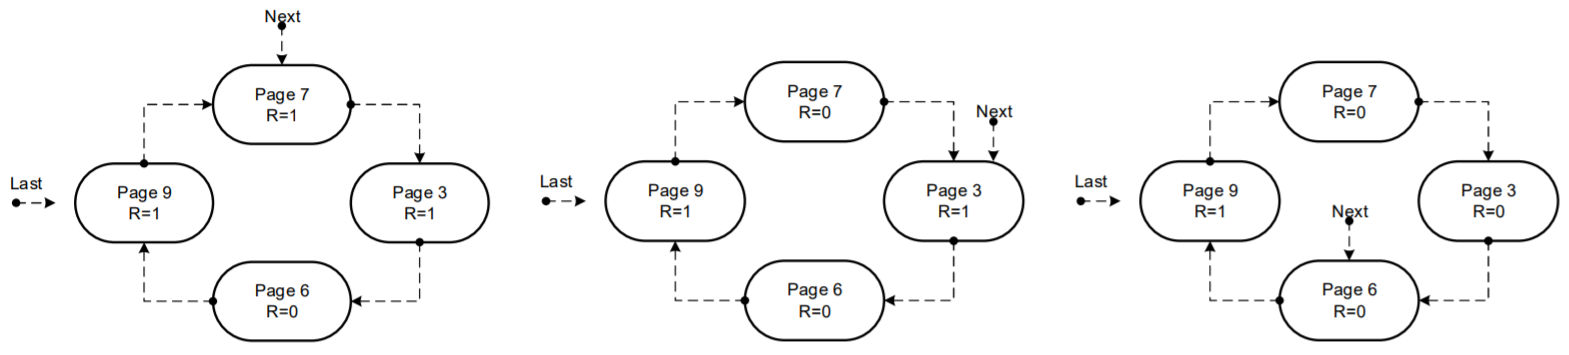
\includegraphics[scale = 0.3]{clock.PNG}\\
\textbf{Not Frequently Used: }Pro Page-Table Eintr. 1 Counter, ersetzt Page min. Counter, - alte, viel gebrauchte Pages bleiben erhalten
\textbf{NFU mit Aging: }4 Bit Counter = Zugr., kein Zugr., Zugr., kein Zugr. 1000$\rightarrow$0100$\rightarrow$1010$\rightarrow$0101
\textbf{Working Set: }R=1: t gesetzt,R=0: aktuelleZeit - t$<$Working Set T$\rightarrow$Nein: Page entfernt, Ja: im Working Set, behalten

\hline
\subsection{In-/Output}
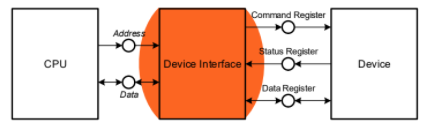
\includegraphics[scale = .5]{io1.PNG}\\
\textbf{Memmory-mapped I/O: }pro Gerät 1 Adressbereich, -1 für Memory, + Einfachheit
\textbf{Port-mapped I/O: }separater Bus, zwei Adressräume (Speicher und Geräte), zwei Instruktionssets, - Komplexität
\textbf{Port-mapped I/O via Speicherbus: }gemeinsamer Bus, \textcolor{red}{zusätzliche Bitleitung für Trennung Speicher|I/O}, Adressraum wird um 1 Bit erweitert\\
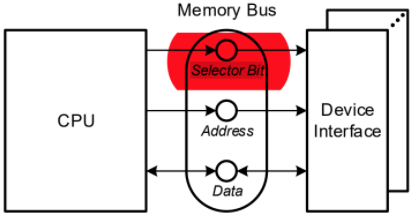
\includegraphics[scale = .5]{io2.PNG}
\subsubsection{Kommunikationsmechanismen}
\textbf{Programmgesteuert/Polling} (Busy Wait = ständig)\\
\textbf{Interruptgesteuert}: \textcolor{green}{Interrupt-Vektor-Tabelle}, Tabelle von Pointern auf Funktionen(von CPU aufgerufen)
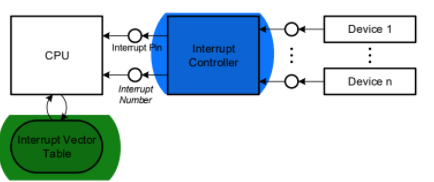
\includegraphics[scale = .5]{io3.PNG}\\
\textbf{Direct Memory Access (DMA)}\\
DMA-Controller steuert Speicherbus anstelle CPU, 1. CPU programmiert DMA für Transfer, 2. DMA lässt Gerät direkt auf Speicherbus kopieren, 3. nach Beendigung setzt DMA Interrupt\\
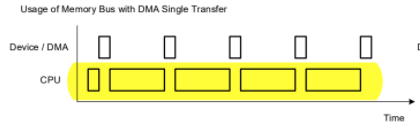
\includegraphics[scale = .5]{singletransfer.PNG}\\
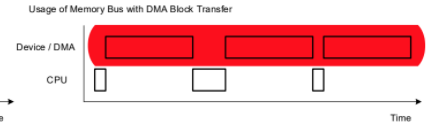
\includegraphics[scale = .5]{blocktransfer.PNG}

\end{multicols*}
\end{document}